\chapter{Results}

\section{Mean Absolute Error (MAE)}
We are using Mean Absolute Error to check the absolute losses in Epouchs. We are plotting a graph between Mean Absolute Error and number of Epouch. This graph will give us more in-sight into the standard error which occures during Training LSTM model.

\begin{figure}[h]
    \centering 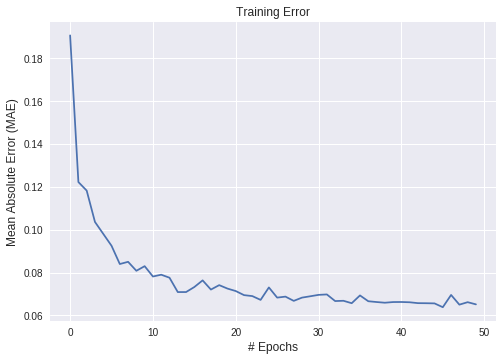
\includegraphics[scale=0.5]{images/mae.png}
    \caption{Mean Absolute Error}
\end{figure}

If everything went to plan, then we'd expect the training error to have gradually decreased over time. In other words, the accuracy of model increase as the model trains.


\section{Single Point Prediction}
Once we have trained our model, it is time to test our model. Initially, we'll test for one particular point. This point will be from our Testing data-set. A good strategy is to keep 80\% of data for training and 20\% for testing.

\begin{figure}[h]
    \centering 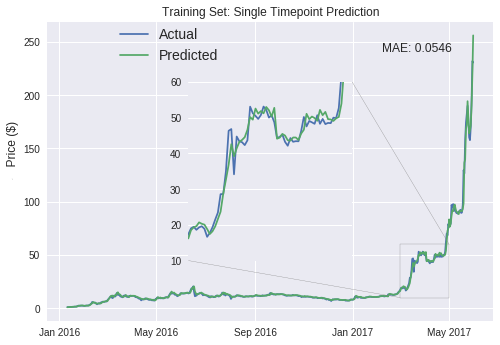
\includegraphics[scale=0.5]{images/s-p.png}
    \caption{Single TimePoint Prediction}
\end{figure}

\section{Calculating Error}
Moving back to the single point predictions, our deep machine artificial neural model looks okay, but so did that boring random walk model. Like the random walk model, LSTM models can be sensitive to the choice of random seed (the model weights are initially randomly assigned). So, if we want to compare the two models, we'll run each one multiple (say, 25) times to get an estimate for the model error. The error will be calculated as the absolute difference between the actual and predicted closing prices changes in the test set.
\begin{figure}[h]
    \centering 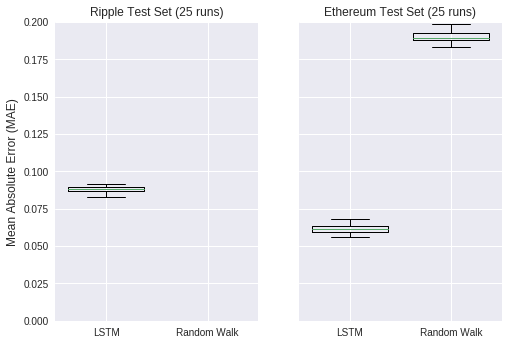
\includegraphics[scale=0.5]{images/error.png}
    \caption{Calculating Error}
\end{figure}
 Those graphs show the error on the test set after 25 different initialisations of each model. The LSTM model returns an average error of about 0.0125 on ripple prices, crushing the corresponding random walk models.
